
% GettingStartedGuideForStudents.tex - Our first LaTeX example!

\documentclass{geocraft-worksheet-multipage}



\usepackage[pdftex,
             pdfauthor={Sarah Zaman \& Dave Ames},
            pdftitle={GeoCraft: Getting Started Guide for Students},
            pdfcreator={LaTeX with hyperref and listings},
            urlbordercolor={1 1 1}]{hyperref}


\begin{document}
\title{Getting Started Guide}
\subtitle{for Students}
\date{}

\maketitle
 
\section*{Step 1}
On the Raspberry Pi desktop click on Menu, Games then Minecraft Pi and
open.\vspace{0.4cm}

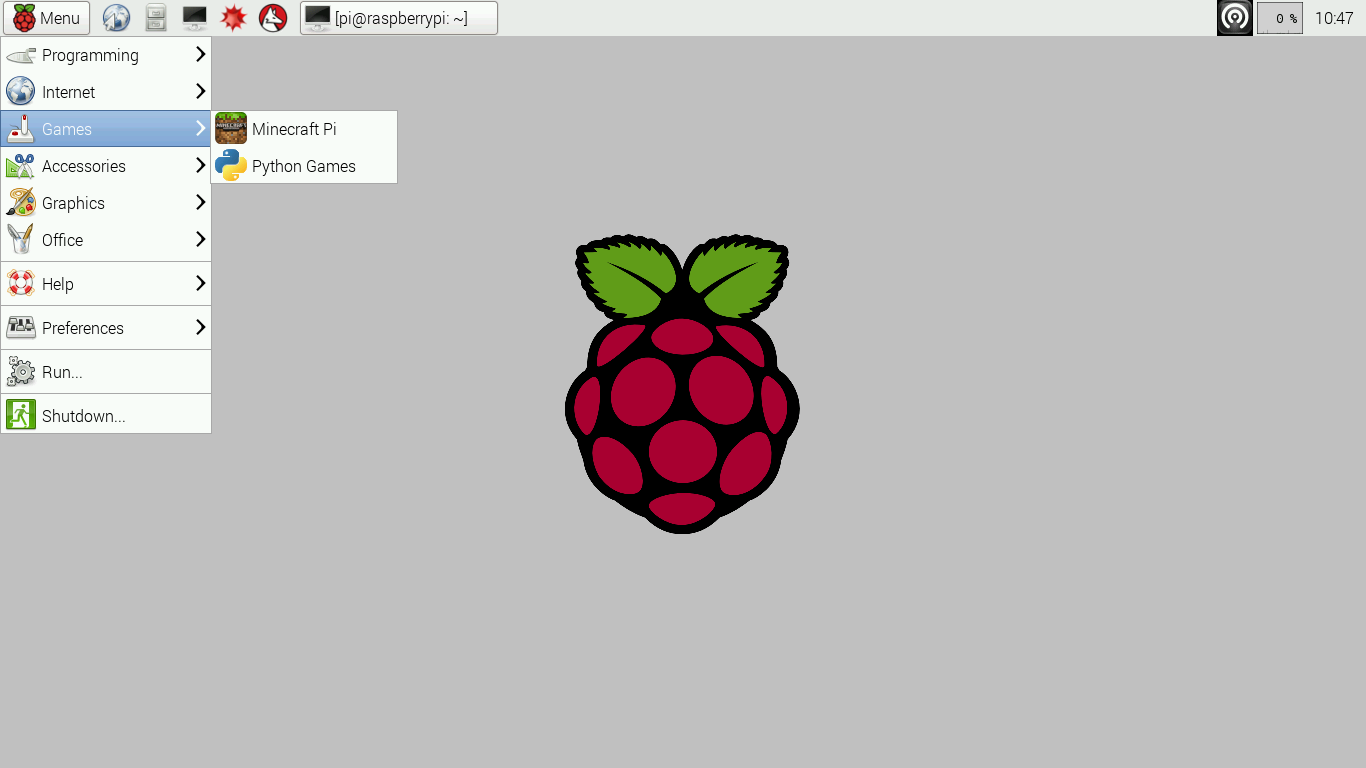
\includegraphics[width=0.5\textwidth]{pic1}\vspace{0.4cm}

Click on Start game then Create New.\vspace{0.4cm}

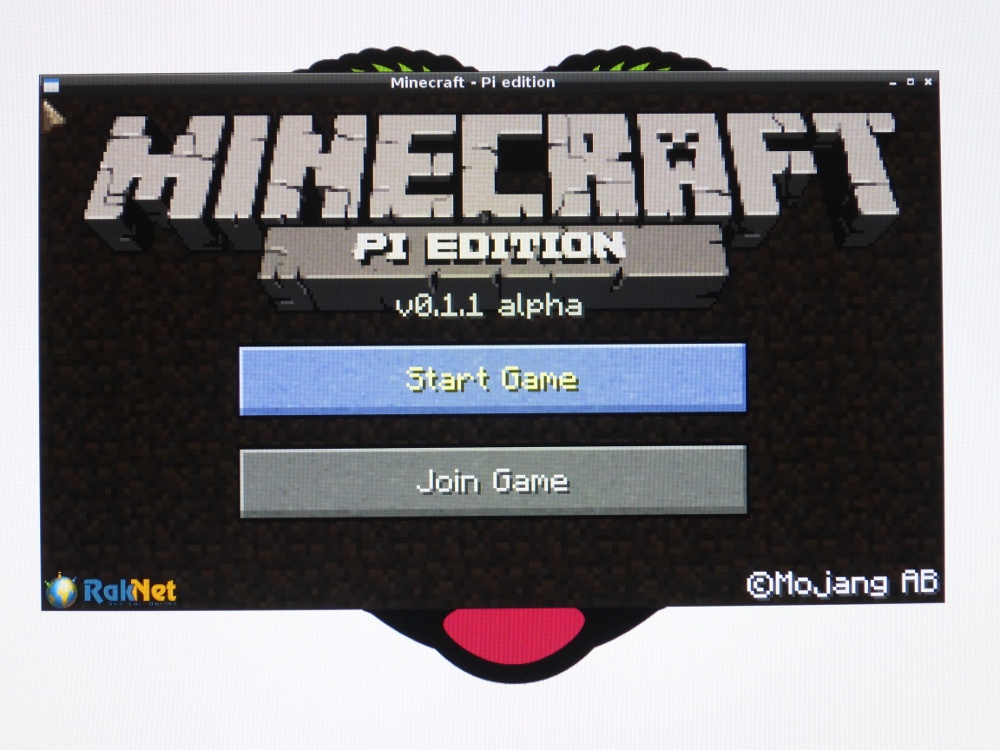
\includegraphics[width=0.5\textwidth]{pic2}\vspace{0.4cm}

\begin{itemize}
\item Have a play in Minecraft if you are unfamiliar.
\item The mouse lets you have a look around.
\item W, A, S and D lets you move forwards, backwards, left and right.
\item Space bar is for jump.
\item Left mouse button destroys blocks.
\item Right mouse button places blocks.
\item E opens the inventory.
\item Escape takes you back.
\end{itemize}

\section*{Step 2}

Now you have played in Minecraft press Escape and then minimise the
window.\\ \vspace{0.4cm}
\textbf{TIP} - Remember it’s the Pi mouse pointer not the Minecraft
mouse pointer you need to use.

\section*{Step 3}

On the Raspberry Pi Desktop click on Menu, Programming then Python
3. \vspace{0.4cm} 

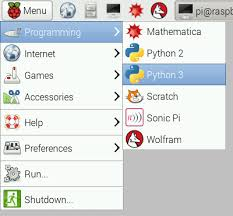
\includegraphics[width=0.5\textwidth]{pic3}\vspace{0.4cm}

The Python Shell window will come up. This is where any bugs in your
program will be reported. \vspace{0.4cm}

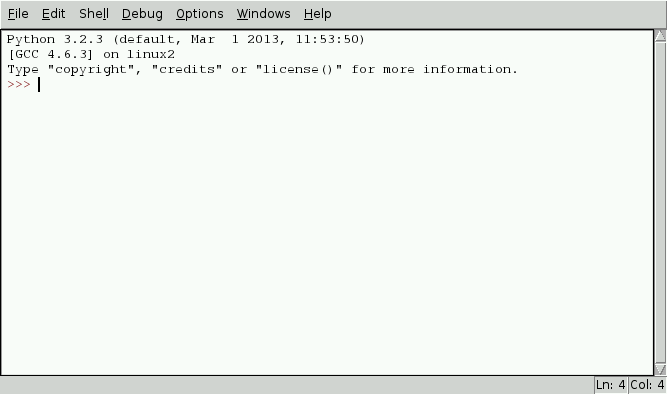
\includegraphics[width=0.5\textwidth]{pic4}\vspace{0.4cm}

Click on File then New Window.This is where you will write your
code.\vspace{0.4cm}

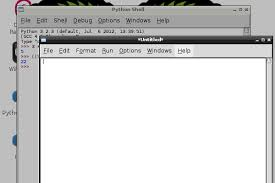
\includegraphics[width=0.5\textwidth]{pic5}\vspace{0.4cm}

Click on File then Save as. Name this file then Save.\vspace{0.4cm}

\textbf{TIP} - This can be saved anywhere in this folder.

\section*{Step 4}

Its time to program.\vspace{0.4cm}

Using the booklet enter the Python code without the numbers.\vspace{0.4cm}

\textbf{TIP} - Remember to use indents and capital letters where it
shows them or your code won’t work. \vspace{0.4cm}

When you have finished click F5 or Run program ,then check for bugs in
the Python Shell window.\vspace{0.4cm}

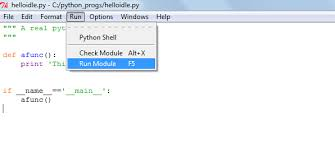
\includegraphics[width=0.3\textwidth]{pic6}\vspace{0.4cm}

Wait a few moments then if Python Shell looks like this then go back
into Minecraft and see if your code has worked. \vspace{0.4cm}


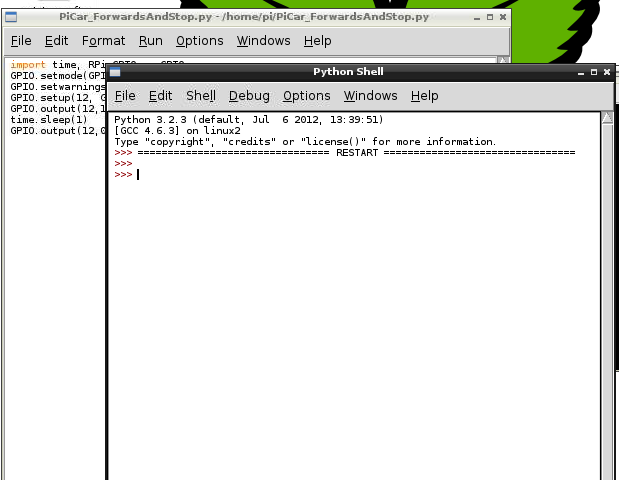
\includegraphics[width=0.5\textwidth]{pic7}\vspace{0.4cm}

If you have bugs which will show up in this window as errors, go back
into your code and check you have correctly typed everything
in. 

\end{document}

%%% Local Variables: 
%%% coding: utf-8
%%% mode: latex
%%% TeX-master: t
%%% End: 
